\section{\Large Realizações}

Para fundamentar esta pesquisa, é necessário abordar a base matemática envolvida e os
resultados essenciais à sua implementação, que foi realizada inicialmente em SageMath, com forte base na implementação presente em \cite{SBSeg21:PM}, e em C++ utilizando-se da biblioteca NTL \footnote{\url{https://libntl.org/}} \cite{shoupNTL}. Ambas implementações estão presentes no repositório no github\footnote{\url{https://github.com/gustavoesteche/ic-bootstraping}}. Primeiramente, serão definidos
os anéis e os corpos utilizados e suas relações, posteriormente, os resultados de como 
efetuar os traços entre os mesmos e como computar as suas bases duais. 
Segundamente, serão definidos os esquemas RLWE e RGSW que foram implementados, 
nos quais o produto externo descrito em \cite{lw23I} é efetuado, sobre o \emph{framework} 
definido pelo mesmo trabalho. Finalmente, será feita uma análise de ruído e complexidade 
destas operações, bem como uma análise sobre sua viabilidade de utilização. 

\subsection{Composição de anéis} 

Considere $m \in \mathbb{Z}$, o objetivo é estudar como compor o anel ciclotômicos coprimos, em um anel ciclotômico resultante $R_m = \mathbb{Q}[X]/\langle\Phi_m(X)\rangle$, onde $\Phi_m(X)$ é o $m$-ésimo polinômio ciclotômico. Como $\mathbb{Q}$ é um corpo e $\Phi_m(X)$ é irredutível sobre $\mathbb{Q}$, por ter raízes primitivas da unidade em $\mathbb{C}$, $R_m$ é um corpo. Além disso, seja $K_m = \mathbb{Q}(\zeta_m)$ a extensão gerada por uma raiz primitiva da unidade de ordem $m$. Pelo isomorfismo $X \mapsto \zeta_m$, temos $R_m \cong K_m$, e portanto decompor $R_m$ equivale a decompor $K_m$. A base canônica (ou de potências) do anel $R_m$ é dada por $B = \{1, X, X^2, \dots, X^{\phi(m)-1}\}$, cujos elementos são linearmente independentes sobre $\mathbb{Q}$. Via isomorfismo, esta base corresponde a $\{1, \zeta_m, \zeta_m^2, \dots, \zeta_m^{\phi(m)-1}\}$ em $K_m$.

Seja $m = \prod_l m_l$, com cada $m_l$ uma potência de primo. Conforme \cite{lyubashevsky2013}, o corpo $K_m$ admite a decomposição:
\begin{equation}
    K_m \cong \bigotimes_l K_{m_l},
\end{equation}
e, analogamente, em termos de anéis polinomiais: $K_m \cong \bigotimes_l \mathbb{Q}[X_l]/\langle\Phi_{m_l}(X_l)\rangle.$

Dessa forma, uma base natural de $K_m$ é o conjunto dos multinômios $\prod_l X_l^{j_l}$ com $0 \leq j_l < \phi(m_l)$, formando a chamada \textit{powerful basis}. Como $\phi(m) = \prod_l \phi(m_l)$, essa base tem o tamanho correto.

A \textit{powerful basis} $\vec{p}$ de $K_m$ é o produto tensorial das bases $\vec{p_l}$ de cada $K_{m_l}$. Os índices do tensor podem ser achatados para formar uma base unidimensional, como discutido em \cite{lyubashevsky2013}. O ponto crucial é entender como efetivar o produto tensorial entre os elementos dos anéis $R_{m_l}$. 

Para isso, usa-se o isomorfismo $X_l \mapsto X^{m/m_l}$, que preserva a relação $\zeta_{m_l} = \zeta_m^{m/m_l}$. Por exemplo, para $m=15$, com $p_3 = \{1, x_3\}$ e $p_5 = \{1, x_5, x_5^2, x_5^3\}$, obtém-se a base $p = \{1, x^3, x^5, x^6, x^8, x^9, x^{11}, x^{14}\}$, como mostrado em \cite{lyubashevsky2013}. Então, de forma generalizada, para realizar o produto tensorial entre os elementos dos anéis $R_{m_l}$, temos:
\begin{equation}
    \prod_{l} \Big( \sum_{i=0}^{\phi(m_l)} a_{il} x^{i m/ml} \Big) \in R_m
\end{equation}

Por fim, como demonstrado em \cite{lyubashevsky2013}, o isomorfismo $\sigma$ de $K_m$ é o produto tensorial dos embeddings canônicos $\sigma^{(l)}$ de cada $K_{m_l}$:

\begin{equation}
    \label{eq:ring_embeddings}
    \sigma\left(\bigotimes_l a_l\right) = \bigotimes_l \sigma^{(l)}(a_l).
\end{equation}

Ou seja, aplicar os homomorfismos antes ou depois do produto tensorial resulta na mesma imagem, o que será explorado a seguir.

\subsection{Traço}
Seja $K \subseteq L $ um extensão de corpo finito e $Aut_K(L)$ o subconjunto de automorfismos
de $L$ que fixam elementos de $K$, ou seja, se $\sigma \in Aut_K(L)$ e $\alpha \in K$, logo $\sigma(\alpha) = \alpha$. Então o Traço de $L$ em $K$ de um elemento $a \in L$ é definido por 
\begin{equation}
    Tr_{L/K}(a) = \sum_{\sigma \in Aut_K(L)} \sigma(a)  
\end{equation} 
Então, computar o traço se resume a encontrar os automorfismos que fixam os elementos.

Sendo $p$ um primo e $n \in \mathbb{Z}^{+}$, considere o anel ciclotômico  
$R_{p^n} = \mathbb{Z}[x]/<\Phi_{p^n}(x)>$. Semelhante a seção anterior, este anel também pode ser escrito como $\mathbb{Z}(\zeta_{p^n})$, onde o isomorfismo é $x \mapsto \zeta_{p^n}$.

Inicialmente, foi encontrado como computar o traço de um elemento $a$ entre os anéis $R_{p^n}$ e $R_{p^{n-1}}$, denotado como $Tr_{R_{p^n}/R_{p^{n-1}}}$.
Observe que o problema foi definido sobre os corpos e não anéis, porém como o automorfismo respeita a estrutura do anel, portanto o traço permanece bem definido. Os automorfismos em anéis ciclotômicos são da forma $X \mapsto X^i$, então, para encontrar os automorfismos basta encontrar os expoentes que satisfazem a propriedade de fixação requerida. 
Vamos separar em dois casos:

\paragraph{Caso 1: $n=1$} 
    Esta discussão é trivial, porque teremos apenas $\varphi(p) = p-1$
    automorfismos, que serão definidos por todos os expoentes coprimos com $p$,
    ou seja $[1,p-1]$. Logo, os automorfismos são $\sigma_i(X) = X^i$.

\paragraph{Caso 2: $n>1$} 
Definimos um conjunto de $\varphi(p^n)/\varphi(p^{n-1}) = p$ automorfismos do anel $\mathbb{Z}[x]/\langle \Phi_{p^n}(x) \rangle$ sobre $\mathbb{Z}[x]/\langle \Phi_{p^{n-1}}(x) \rangle$, dados por:
\[
\sigma_k(x) = x^{k p^{n-1} + 1}, \quad 0 \leq k \leq p-1.
\]
Se $g(x) \in R_{p^{n-1}}$, ou seja, $g(x) = \sum_{i=0}^{\varphi(p^{n-1})} b_i \zeta_{p^{n-1}}^i$. Usando $\zeta_{p^{n-1}} = \zeta_{p^n}^p$, $\sigma_k(g(x))$ pode ser escrito como:
\[
\sigma_k(g(x)) = \sum_i b_i x^{pi(k p^{n-1} + 1)} = \sum_i b_i x^{p i k p^{n-1}} x^{pi}.
\]

Como $x^{p i k p^{n-1}} = (x^{p^n})^{ik} \equiv 1 \mod \Phi_{p^n}(x)$, segue que $\sigma_k(g(x)) = g(x)$. Portanto, os automorfismos $\sigma_k$ \emph{fixam} o subanel $R_{p^{n-1}}$.

Seja $f(x)$ um polinômio em $R_{p^n}$ escrito como 
$
f(x) = \sum_{i=0}^{\varphi(p^n)/p} x^{pi} \sum_{j=0}^{p-1} a_{ij} x^j.
$ podemos simplificar a atuação do traço de $R_{p^n}$ para $R_{p^{n-1}}$:

\[
\sum_{k=0}^{p-1} \sigma_k(f(x)) = p \sum_{i=0}^{\varphi(p^n)/p} x^{pi} a_{i0}.
\]
Esse traço pode ser aplicado recursivamente por uma torre:
$
R_{p^n} \longrightarrow R_{p^{n-1}} \longrightarrow \cdots \longrightarrow \mathbb{Z},
$
permitindo computar traços intermediários até o corpo base, ou até o corpo necessário, operação implementada em SageMath.

Ademais, foram obtidas expressões explícitas para os traços parciais $\mathrm{Tr}_{K/K_{12}}$ e $\mathrm{Tr}_{K/K_{13}}$, fundamentais para o \textit{framework} de \textit{batch bootstrapping} apresentado em \cite{lw23I}. Seja $K = K_1 \otimes K_2 \otimes K_3$ e $K' = \bigotimes_{l \neq q} K_l$, então, para $a = \bigotimes_l a_l \in K$, usando a equação [\ref{eq:ring_embeddings}] foi demonstrado que:

\begin{equation}
    \mathrm{Tr}_{K/K'} (a) = \left( \bigotimes_{l \neq q} a_l \right) \cdot \mathrm{Tr}_{K_q/\mathbb{Q}} (a_q)
\end{equation}

Essa fórmula permite computar o traço parcial removendo um dos fatores do produto tensorial de corpos, simplificando significativamente sua implementação algébrica, que foi usado para critério de confirmação da solução polinômial e pode ser utilizada no futuro para otimização da implementação proposta, foi implementada em SageMath.

Em vias de fato, os tensores são uma das representações do que 
na realidade é representado por um polinômio $f(x) \in K$. No desenvolvimento a seguir vamos tratar novamente do caso onde queremos eliminar um corpo do traço, ou seja,
fixar os elementos dos outros corpos. Tome os mesmos corpos definidos anteriormente. Como $K$ é dado por um produto tensorial, para $f(x) \in K$ temos:  
$$
f(x) = \sum_i^{\phi(m1)-1} a_i x^{im_2m_3} \times \sum_j^{\phi(m2)-1} b_j x^{jm_1m_3} \times \sum_k^{\phi(m3)-1} c_i x^{km_1m_2}
$$ 
onde cada termo estava originalmente em $K_1,K_2, K_3$ respectivamente. Assuma sem perda de generalidade que queremos fixar os elementos dos dois primeiros corpos.
logo, o automorfismo $a$ tem a forma: 
$$
 x^{a(im_2m_3 + jm_1m_3)} = x^{im_2m_3 + jm_1m_3}
$$
Então $a m_2 m_3 \equiv m_2 m_3 $ e $a m_1 m_3 \equiv m_1 m_3$, para isso $a = k \times m_1 m_2$. Porém, é importante que $a m_1 m_3 \not\equiv m_1 m_3$, portanto
temos que remover esses múltiplos apropriadamente. A solução pode ser vista no seguinte pseudocódigo:

\begin{algorithm}[H]
\caption{Cálculo dos automorfismos}
\KwIn{Inteiros $m$, $p$, $n$}
\KwOut{Lista de automorfismos}

$rest \gets \{\, i \in [0, p-1] \mid i \neq k \,\}$ \;
$aut \gets \emptyset$ \;

\For{$i \gets 0$ \KwTo $p^{n-1} - 1$}{
    \ForEach{$j \in rest$}{
        $a \gets (i \cdot p + j) \cdot m / p^n + 1$ \;
        adiciona $a$ a $aut$\;
    }
}
\Return $aut$
\end{algorithm}

Tais automorfismos são aplicados na definição de traço para seu cálculo na implementação. Esta função foi implementada em SageMath e C++.

\subsection{Dual}

O cálculo da base dual dos corpos trabalhado é essencial para o empacotamento proposto em \cite{lw23I}. Seja $K = \mathbb{Q}(\zeta_m)$ e $B = \{b_j\}$ uma base de $K$ sobre $\mathbb{Q}$. Define-se a base dual $B^v = \{b_j^v\}$ por:
\[
\mathrm{Tr}(b_i b_j^v) = \delta_{ij}
\]
O que implica que qualquer elemento $a \in K$ satisfaz $a_j = \mathrm{Tr}(a b_j^v)$.

No caso da base canônica $[x^0,x^1, \dots, x^{\varphi(p^n)-1}]$, o problema se reduz a encontrar elementos $k_i$ que satisfaçam:
\[
\mathrm{Tr}(x^i k_j) = \delta_{ij} \cdot p^n
\]
Utiliza-se para isso os polinômios $k_i = x^{p^n - i} - x^{p^{n-1} - i}$, com base na fórmula:
\[
\mathrm{Tr}(x^j) =
\begin{cases}
\varphi(p^n) & \text{se } j \equiv 0 \pmod{p^n} \\
-p^{n-1} & \text{se } j \equiv 0 \pmod{p^{n-1}} \wedge j \not\equiv 0 \pmod{p^n} \\
0 & \text{caso contrário}
\end{cases}
\]

Esse $k_i$ satisfaz $\mathrm{Tr}(x^i k_i) = p^n$, mas falha para o par $(i, i + p^{n-1})$. Para corrigir, redefine-se:
\[
k_{i + p^{n-1}} := k_{i + p^{n-1}} + k_i
\]
Garantindo que $\mathrm{Tr}(x^j k_i) = 0$ para $j \neq i$ e $\mathrm{Tr}(x^i k_i) = p^n$.

Assim, temos o seguinte algoritmo para computar a base dual canônica:

\begin{algorithm}[H]
\caption{\texttt{canon\_dbasis(p, n)}}
\KwIn{Primo $p$, inteiro $n \geq 1$}
\KwOut{Base dual canônica de $\mathbb{Q}(\zeta_{p^n})$}
$f \gets \Phi_{p^n}(x)$ \\
Inicializa vetor $l$ com zeros em $\mathbb{Q}[x]/(f)$ \\
\For{$i \gets 0$ \KwTo $p^{n-1} - 1$}{
    $l[i] \gets (x^{p^n - i} - x^{p^{n-1} - i}) \bmod f$
}
\For{$i \gets p^{n-1}$ \KwTo $\varphi(p^n) - 1$}{
    $l[i] \gets (l[i] + l[i - p^{n-1}])/p^n$
}
\Return{$l$}
\end{algorithm}

Cada elemento da base resultante tem norma infinita $\leq 2(p-1)/p^n$, propriedade que será útil na análise de ruído em aplicações criptográficas. A implementação foi feita em SageMath e C++.  


\subsection{RLWE e RGSW}
Nesta seção os esquemas e seus parâmetros serão apresentados tais como descritos em \cite{lw23I} com 
os detalhes específicos utilizados na implementação. Ambos esquemas tem sua segurança baseada no problema Learning With Errors(LWE), problema creditado como difícil \cite{BrakerskiEtAl2013}. Porém, provas e discussões sobre sua dificuldade e definições de parâmetros se estendem juntamente a padronização do NIST \cite{Balbas2021}. 

É necessário a introduzir a operações de decomposição. Tome o vetor $g^\top = (1, 2, \dots, 2^{\ell-1})$ e a matriz definida por $G = g^\top \otimes I_2$.  

\begin{lemma}[lema 2.3 \cite{lw23I}]
Dado um inteiro $q$, seja $\ell = \lceil \log q \rceil$, $\mathbf{g}^\top = (1, 2, \dots, 2^{\ell - 1})$ e uma base fixa $\mathbb{Z}_q$ de $\{ \mathbf{b}_1, \dots, \mathbf{b}_n \}$ de $\mathcal{O}_K / q \mathcal{O}_K$. Então, existe uma função aleatória e eficientemente computável
\[
\mathbf{g}^{-1} : \mathcal{O}_K / q \mathcal{O}_K \rightarrow \mathcal{O}_K^\ell
\]
tal que a saída da função, $\mathbf{x} \leftarrow \mathbf{g}^{-1}(a)$, sempre satisfaz $\langle \mathbf{g}, \mathbf{x} \rangle = a \bmod q$.

Mais especificamente, se $a = a_1 \mathbf{b}_1 + \dots + a_n \mathbf{b}_n$ onde $a_i \in \mathbb{Z}_q$ e $\mathbf{x}_i \leftarrow \mathbf{g}^{-1}(a_i)$ (onde a função $\mathbf{g}^{-1}(\cdot)$ é definida no Lema~2.1), então:
\[
\mathbf{x} = \mathbf{x}_1 \mathbf{b}_1 + \dots + \mathbf{x}_n \mathbf{b}_n
\]
e cada vetor $\mathbf{x}_i \in \mathbb{Z}_q^\ell$ é sub-Gaussiano com parâmetro $O(1)$.
\end{lemma}

Perceba que é possível definir a mesma função para $G$, $G^{-1}$. A mesma se baseia na aplicação da anterior nas devidas linhas tal que $\langle \mathbf{G}, \mathbf{G^{-1}(x)} \rangle = x$.

Abaixo estão presentes os parâmetros utilizados nos esquemas:

\begin{itemize}[itemsep=0pt, parsep=0pt]
    \item[-] $\lambda$: o parâmetro de segurança
    \item[-] $\mathcal{R}$: o anel ciclotômico $\frac{\mathbb{Z}[x]}{<\Phi_{m}(x)>}$
    \item[-] $Q$: o módulo inteiro onde as cifras operam
    \item[-] $\mathcal{R}_{Q}$: o anel quociente $\mathcal{R}/Q\mathcal{R}$
    \item[-] $\mathcal{D_{\sigma}}$: Distribuição gaussiana discreta de ruído sobre $\mathcal{R}$ com desvio padrão $\sigma$.
    \item[-] $l$ = $\log_t(Q)$ 
    \item[-] $t$: o módulo da mensagem no RLWE, para o RGSW utilizado considera-se $t=2$
\end{itemize}

\subsubsection{Esquema RLWE}

\begin{itemize}[itemsep=0pt, parsep=0pt]
    \item[-] \textbf{KeyGen}($1^{\lambda}$): Amostre uma chave secreta $s \leftarrow \mathcal{R}_Q$
    \item[-] \textbf{Enc}(sk, $\mu \in \mathcal{R}_t$): Amostre um elemeto uniforme do anel $a \leftarrow \mathcal{R}_q$ e
um erro $e \leftarrow \mathcal{D_{\sigma}}$. Retorne um criptograma definido por 
    $$
    c := (a, sa + \left\lfloor \frac{Q}{t} \right\rceil \mu + e)
    $$
    \item[-] \textbf{Dec}(c, sk): O algoritmo retorna um elemento $\mu \in \mathcal{R}_t$ definido por:
    $$
        \mu = \left\lfloor t \left\langle (1,-s),c \right\rangle/Q \right\rceil  \pmod{t}  
    $$
\end{itemize}

O ruído de um criptograma $c$ que ecriptma $\mu$ sobre a chave secreta $s$ pode ser definido por 
$$Err_\mu(c) = \left\langle (-s,1), c \right\rangle- \left\lfloor \frac{Q}{t} \right\rceil \mu$$

\subsubsection{Esquema RGSW}

\begin{itemize}[itemsep=0pt, parsep=0pt]
    \item[-] \textbf{KeyGen}($1^{\lambda}$): Amostre uma chave secreta $s \leftarrow \mathcal{R}_Q$.
    \item[-] \textbf{Enc}(sk, $\mu \in \mathcal{R}$): Amostre um vetor uniformemente $\mathbf{a} \leftarrow \mathcal{R}_Q^{2\ell}$ e um vetor de ruído $e \leftarrow D_{\sigma}^{2\ell}$. Retorne um 
    criptograma definido por $C := \begin{pmatrix} s \mathbf{a}^\top + \mathbf{e}^\top \\ \mathbf{a}^\top \end{pmatrix} + \mu \mathbf{G} \in R_Q^{2 \times 2\ell}$
    \item[-] \textbf{Dec}(c, sk): O algortimo retorna um elemento $\mu \in \mathcal{R}/2\mathcal{R}$:
    $$ 
    \mu = \left\lfloor \left\langle (1,-s),_{(2\ell -1)}c \right\rangle/Q \right\rceil  \pmod{2}  
    $$
    
\end{itemize}

O ruído de um criptograma $C$ que encripta a mensagem $\mu$ sobre a chave secreta $sk = (1, -s)^T$ pode ser
definido por $Err_\mu(C) = e^T = sk^T \cdot C - \mu \cdot sk^T \cdot G$ 

\paragraph{Operações}

\begin{itemize}
    \item[-] \textbf{Soma Homomórfica} $C_1 \boxplus C_2 $: Recebe dois criptogramas RGSW $C_1, C_2$ cifrados sobre a mesma chave e retorna $C_1 \boxplus C_2 := C_1 + C_2$. 
    O novo criptograma obtido cifra a soma das mensagens ($\mu_1, \mu_2$):
    $$
    C_1 + C_2 = \begin{pmatrix} s (\mathbf{a_1}^\top + \mathbf{a_2}^\top) + \mathbf{E}^\top \\ \mathbf{a_1}^\top + \mathbf{a_2}^\top \end{pmatrix} + (\mu_1 + \mu_2) \mathbf{G}
    $$
    \item[-] \textbf{Multiplicação Homomórfica} $C_1 \boxdot C_2$: Recebe dois criptogramas RGSW $C_1, C_2$ cifrados sobre a mesma chave e retorna $C_1 \boxdot C_2 := C_1 \mathbf{G^{-1}}(C_2)$. 
    O novo criptograma obtido cifra a multiplicação das mensagens ($\mu_1, \mu_2$): 
    $$
    C_1 \mathbf{G^{-1}}(C_2) = \begin{pmatrix} s \mathbf{a_1}^\top + \mathbf{e_1}^\top \\ \mathbf{a_1}^\top \end{pmatrix} \mathbf{G^{-1}}(C_2)  + (\mu_1) \begin{pmatrix} s \mathbf{a_2}^\top + \mathbf{e_2}^\top \\ \mathbf{a_2}^\top \end{pmatrix} + \mu_1 \mu_2 \mathbf{G}
    $$
    $$
        = \begin{pmatrix} s (\mathbf{a_1}^\top \mathbf{G^{-1}}(C_2) + \mu_1 \mathbf{a_2}^\top) + \mathbf{e_1}^\top \mathbf{G^{-1}}(C_2) + \mu_1 \mathbf{e_2}^\top \\ \mathbf{a_1}^\top + \mu_1 \mathbf{a_2}^\top \end{pmatrix}  + \mu_1 \mu_2 \mathbf{G}
    $$
    \item[-] \textbf{Produto Externo} $C_1 \boxtimes c_2 $: Recebe um criptogramas RGSW e um RLWE $C_1, C_2$ respectivamente cifrados sobre a mesma chave e retorna $C_1 \boxtimes C_2 := C_1 \mathbf{g^{-1}}(c_2)$. 
    O novo criptograma obtido cifra a multiplicação das mensagens ($\mu_1, \mu_2$) pelo processo análogo ao anterior, suprimido para conscisão.
\end{itemize}

Para checar a implementação dos esquemas e cada uma das operações descritas, aquém da multiplicação homomórfica, acesse o github \footnote{\url{https://github.com/gustavoesteche/ic-bootstraping}} 

\subsection{Empacotamento de \textit{plaintext} e \textit{ciphertext}}

Neste momento a seção 4 de \cite{lw23I} é tomada como base, cujo as 
operações foram implementadas em SageMath e C++. A única operação não implementeada foi a multiplicação entre criptogramas RGSW, afinal foge do escopo deste trabalho. A seguir, tome convenções necessárias para o resto do trabalho, tome $\rho = \varphi(p_2^{n_2})$, $\rho' = p_2^{n_2}$ com base $v_i$ e dual $v_i^{v}$; $\tau = \varphi(p_3^{n_3})$, $\tau' = p_3^{n_3}$ com base $w_i$ e dual $w_i^{v}$; $\delta_i^{(j)}$ representa a $i$-ésima componente do ruído da mensagem $\mu_i^{(j)}$ empacotada e cifrada em RGSW; $e_i^{(j)}$ é a $i$-ésima componente do ruído da mensagem $d_j$ resultante empacotada em RLWE.

\paragraph{Nota:} A única diferença da implementação para o proposto teoricamente é que para os plaintexts e ciphertexts, seus elementos vão ser armazenados sempre em $\mcR$ ao invés de ocasionalmente em $\mcR_1 \otimes \mcR_2^\vee \otimes \mcR_3$ ou $\mcR_1 \otimes \mcR_2 \otimes \mcR_3^\vee$. Por exemplo, para o criptograma  $a \in \mathcal{R}_1 \otimes \mathcal{R}_2^\vee \otimes \mathcal{R}_3$, vamos armazenar o criptograma $aP \in \mcR$ onde $P = \rho$. Esta multiplicação garante que o elemento tem representação única em $\mcR$ e facilita a implementação.

Surge uma dúvida natural, \textbf{Por que não empacotar as mensagens em um criptograma?}
O ruído acaba crescendo exponencialmente ao realizar múltiplos produtos externos consecutivamente. Emprestando um resultado da sessãoi seguinte, se decidirmos empacotar mensagens a expressão de um produto externo será: $Tr_{K/K_{13}} (e_1g^{-1}(c_2) + \mu_1 e_2) + e'$

Onde $e_1, e_2$ são os ruídos do criptograma RGSW e RLWE respectivamente. Como o ruído não possui nenhuma propriedade especial em relação as bases $v_i, w_i$ é válido afirmar que a sua norma vai crescer proporcional a um fator $\phi(p_2^{n_2})$. Portanto, após $k$ aplicações de produto externo, a norma final será limitada com um fator de $\approx \phi(p_2^{n_2})^{k/2} \phi(p_3^{n_3})^{k/2}$
que é exponencial. Tal crescimento pode ser verificado via o gráfico a seguir:

\begin{figure}[H]
    \centering
    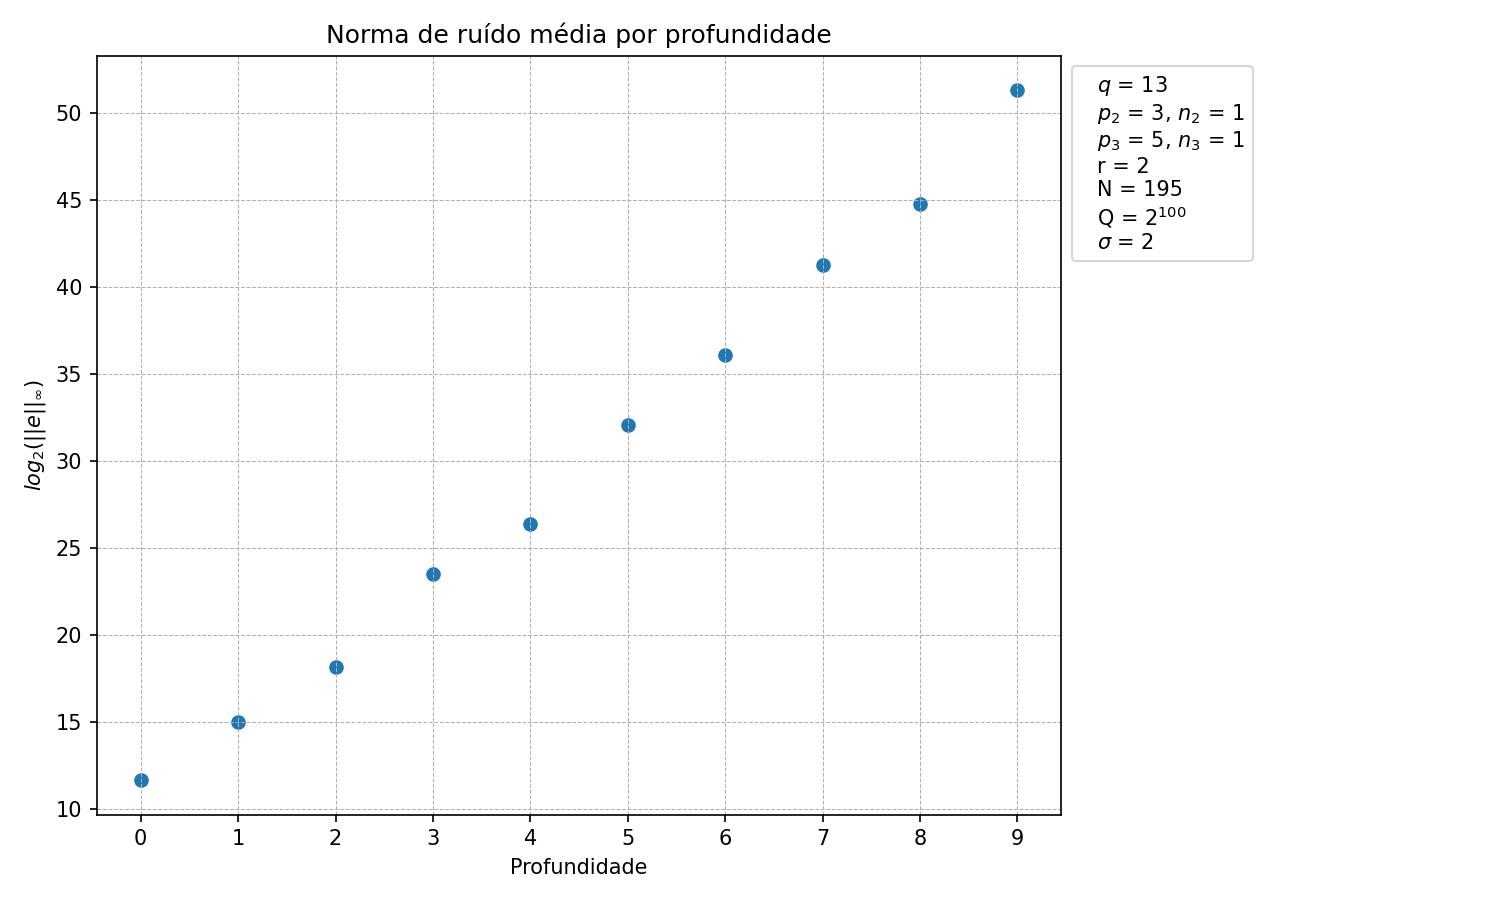
\includegraphics[width=0.7\textwidth]{sections/images/wrong_packing.jpg}
    \caption{Crescimento do ruído pela quantidade de produtos externos com empacotamento ingênuo.}
    \label{fig:wrong_packing}
\end{figure}


\subsection{Análise de Ruído das operações}

Nesta seção estão as análises do crescimento de ruído das operações entre criptogramas RLWE e RGSW.
\subsubsection*{Soma Homomórfica $C_1 \boxplus  C_2$}
O ruído dessa operação pode ser calculado por:
$$
Err(C_1 \boxplus  C_2) = sk^T(C_1 + C_2) - (\mu_1 + \mu_2)sk^TG
$$
Organizando,
$$
Err(C_1 \boxplus  C_2) = sk^T(C_1) - (\mu_1)sk^TG + sk^T(C_2) - (\mu_2)sk^TG = e_1^T + e_2^T 
$$

\subsubsection{Multiplicação Homomórfica $C_1 \boxdot C_2$}
O ruído desta operação pode ser calculado por
$$
Err(C_1 \boxdot C_2) = sk^\top(C_1G ^{-1}(C_2)) - (\mu_1\mu_2)sk^\top \mathbf{G}
$$
Expandindo a expressão encontra-se:
$$
Err(C_1 \boxdot C_2) = (1,-s) \begin{pmatrix} s \mathbf{a}_1^\top + \mathbf{e}_1^\top \\ \mathbf{a}_ 1^\top \end{pmatrix}G ^{-1}(C_2) + \mu_1(1,-s)\begin{pmatrix} s \mathbf{a}_2^\top + \mathbf{e}_2^\top \\ \mathbf{a}_ 2^\top \end{pmatrix}
$$
Simplificando, finalmente:
$$
Err(C_1 \boxdot C_2) = \mathbf{e}_1^\top G ^{-1}(C_2) + \mu_1 \mathbf{e}_2^\top
$$

O produto externo padrão entre RGSW e RLWE pode ser calculado por

$$C_1 \boxtimes c_2 = \begin{pmatrix} s \mathbf{a}_1^\top + \mathbf{e}_1^\top \\ \mathbf{a}_ 1^\top \end{pmatrix}g^{-1}(c_2) + \mu_1\mathbf{G}g^{-1}(c_2)$$ 
$$=\begin{pmatrix} s \mathbf{a}_1^\top g^{-1}(c_2) + \mathbf{e}_1^\top g^{-1}(c_2) \\ \mathbf{a}_ 1^\top g^{-1}(c_2) \end{pmatrix} + \begin{pmatrix} s a_2 \mu_1 + \mu_1 \mu_2 \frac{Q}{B} + \mu_1 e_2 \\ a_2 \mu_1 \end{pmatrix} $$
$$=\begin{pmatrix} s ( \mathbf{a}_1^\top g^{-1}(c_2) + a_2\mu_1) + \mu_1\mu_2\frac{Q}{B} +  \mathbf{e}_1^\top g^{-1}(c_2) +\mu_1 e_2 \\ \mathbf{a}_ 1^\top g^{-1}(c_2) + a_2 \mu_1 \end{pmatrix}$$
Finalmente, o ruído é calculado por:
$$
Err(C_1 \boxtimes c_2) = \mathbf{e}_1^\top g^{-1}(c_2) +\mu_1 e_2  
$$
Dessa forma, a sua norma infinita deve ser
$$
||Err(C_1 \boxtimes c_2)||_\infty < 2\ell N||e_1||_\infty + \mu_1 ||e_2||_\infty 
$$

\subsubsection{Subgaussiana}
Para a análise de ruído 'justa' é preciso utilizar que parte das variáveis aleatórias trabalhadas são limitadas por distribuições 
subgaussianas. A intuição é de que podemos encontrar um limite superior probabilístico utilizando a desigualdade de Markov se soubermos
a distribuição que rege a variável aleatória. 

\begin{definition}
    Para \( s > 0 \), define-se a função Gaussiana \( \rho_s : H \to (0,1] \) por
\[
\rho_s(\mathbf{x}) = \exp\left(-\pi \|\mathbf{x}\|_2^2 / s^2\right).
\]
A distribuição Gaussiana contínua \( D_s \) é obtida pela normalização de \( \rho_s \), com densidade \( s^{-n} \cdot \rho_s(\mathbf{x}) \).

Define-se também que uma variável aleatória \( X \in \mathbb{R} \) é \( \delta \)-subgaussiana com parâmetro \( s > 0 \) se, para todo \( t \in \mathbb{R} \),
\[
\mathbb{E}[\exp(2\pi t X)] \leq \exp(\delta + \pi s^2 t^2).
\]

\end{definition}

Agora tome as seguintes propriedades presentes em \cite{lyubashevsky2013} e \cite{lw23I}.

\begin{lemma}[Lema 3.2 \cite{lw23I}]
    \textit{Para quaisquer cifras RGSW} $\mathbf{C}_1, \mathbf{C}_2$ \textit{que cifram} $\mu_1, \mu_2$ \textit{com termos de erro} $\mathbf{e}_1, \mathbf{e}_2$ \textit{respectivamente, temos o seguinte:}

    \[
    \text{Err}(\mathbf{C}_1 \boxplus \mathbf{C}_2) = \mathbf{e}_1^\top + \mathbf{e}_2^\top.
    \]

    \[
    \text{Err}(\mathbf{C}_1 \boxtimes \mathbf{C}_2) = \mathbf{e}_1^\top \cdot \mathbf{G}^{-1}(\mathbf{C}_2) + \mu_1 \cdot \mathbf{e}_2^\top.
    \]

    \textit{Além disso, suponha que} $\mathbf{G}^{-1}$ \textit{é amostrado com respeito a alguma base} $\mathbb{Z}$ \textit{de} $\mathcal{R}$, \textit{isto é,} $\mathbf{B} = \{ \mathbf{b}_1, \dots, \mathbf{b}_n \}$, \textit{tal que} $\max_{i \in [n]} \{ \| \sigma(\mathbf{b}_i) \|_\infty \} \leq 1$ \textit{como no Lema 2.3. Então os seguintes fatos valem:}

    \begin{itemize}
    \item Denote $\mathbf{e}_1^\top \cdot \mathbf{G}^{-1}(\mathbf{C}_2)$ como $\mathbf{e}^\top = (e_1, \dots, e_{2\ell})$. Então cada entrada de $\mathbf{e}$ é uma variável aleatória independente.

    \item $\|\sigma(\mathbf{e})\|_\infty$ é limitada superiormente por uma variável sub-Gaussiana com parâmetro $O(r)$, para algum $r > 0$ tal que $r \leq \sqrt{N \cdot \log Q} \cdot \|\sigma(\mathbf{e}_1)\|_\infty$.
    \end{itemize}
\end{lemma}

\begin{lemma}
    Seja uma variável aleatória $X$ de distribuição gaussiana de parâmetros $(\mu = 0, \sigma)$, esta variável é limitada superiormente
    por um subgaussiana de parâmetro mínimo $\sqrt{2\pi}\sigma$
\end{lemma}

Com o último lema, garantimos que a amostragem gaussiana do erro reflete em uma variável subgaussiana. Logo, passamos para uma análise dos ruídos acumulados pelo resto das operações.

\subsubsection{Key Switch}
O algoritmo de key-switch, tem como função a troca de chave de um criptograma cifrado
em uma chave antiga $s'$, para uma chave nova $s$, o que aumenta o ruído gerado na cifra, vamos verificar quanto.
Para que o algortimo seja realizado corretamente, é necessário 
que seja passado como parâmetro a \textit{lower half} de um criptograma $RGSW_s(s')$, ou seja, é necessário assumir 
que o RGSW tem segurança circular.

Seja então $d \in \text{RLWE}_{s'}(\mu)$ e $d = (a, b)$, e queremos então um criptograma de $\mu$ cifrado em $\text{RLWE}_{s}$.
Considere então $K$ a \textit{lower half} de um criptograma $RGSW_s(s')$. O objetivo então é encontrar o ruído gerado por, 
$$
[0,b] - K \times g^{-1}(a)
$$
Como $K$ é a parte inferior de $RGSW_s(s')$ considere $K = (A, As + gs' + \mathbf{e}_{KS}) \in \mathcal{R}_Q^{2 \times \ell}$. Desenvolvendo,

$$
-(g^{-1}(a) \times A), -(g^{-1}(a) \times A) s + \mu \frac{Q}{B} + E - \mathbf{e}_{KS} g^{-1}(a)
$$
Note que o vetor obtido é um criptograma valido $\in \text{RLWE}_{s}(\mu)$ com ruído 
$E - \mathbf{e}_{KS} g^{-1}(a)$ que possui norma infinita correspondente:
$$
||Err(KS(d))||_\infty < ||Err(d)||_\infty + N\ell ||\mathbf{e}_{KS}||_\infty
$$
No teorema 4.6 de \cite{lw23I}, assume-se que $Err(d)$ e $\mathbf{e}_{KS} g^{-1}(a)$ são subgaussianas com um mesmo parametro $B$, o que é coerente visto que a magnitude do ruído do key-switch deve ser muito menor do que a da mensagem $d$. O key switch foi implementado em SageMath e C++.

\subsubsection{Eval-Trace}

Para facilitar a análise de ruído do algoritmo 4.1 de \cite{lw23I}, considere o mesmo
algoritmo simplificado, para o efeito da acumulação do ruído ser mais visível, a variável $d$ terá um 
índice que representa seu degrau na torre de extensão. 

\begin{algorithm}[H]
\caption{(RLWE)-Eval-Tr\(_{K/K_{13}}\) com a estrutura de torre}
\SetKwInOut{Input}{Entrada}
\SetKwInOut{Output}{Saída}

\Input{
\begin{itemize}
  \item \(c = (b, a) \in (\mathcal{R}_1 \otimes \mathcal{R}_2 \otimes \mathcal{R}_3)^2\) que encripta uma mensagem \(\mu \in \mathcal{R}_1 \otimes \mathcal{R}_2 \otimes \mathcal{R}_3\) sob um segredo \(s \in \mathcal{R}\).
  \item \(\{\text{evk}^{(\sigma)}\}_{\sigma \in \bigcup_{i=1}^{t-1} \text{Gal}(E_i/E_{i+1})}\), e \(\text{evk} \in \text{RGSW}_s(P^{-1} \cdot s) \in \mathcal{R}^2\).
\end{itemize}
}
\Output{
\(c_{out} \in \text{RLWE}_s(\text{Tr}_{K/K_{13}}(\mu))\).
}

Inicialize \(c = (b, a)\), defina \(\bar{a} = P \cdot a\) \\
Calcule \(d_0 = \text{evk} \boxtimes (0, \bar{a})\) \\
\For{\(i = 1\) até \(t - 1\)}{
  Calcule \(d_{i+1} = \sum_{\sigma \in \text{Gal}(E_i/E_{i+1})} \text{KS}( \sigma(d_i), \text{evk}^{(\sigma^{-1})})\)\\
}
Retorne \((\text{Tr}_{K/K_{13}}(b), 0) - d_n\) 

\end{algorithm}
Assuma sem perda de generalidade que o traço realizado é $K \rightarrow K_{13}$.
Começaremos analisando a recurssão do loop na linha 4:
$$
d_{i+1} = \sum_{\sigma \in \text{Gal}(E_i/E_{i+1})} \text{KS}( \sigma(d_i), \text{evk}^{(\sigma^{-1})})
$$
Então, utilizando a expressão do erro do key-switch:
$$
Err(d_{i+1}) = \sum_{\sigma \in \text{Gal}(E_i/E_{i+1})} Err(\sigma(d_i)) - e_{KS}^{\sigma} g^{-1}(d_i[0])
$$
Perceba que $Err(\sigma(d_i)) = \sigma(Err(d_i))$ e que o segundo termo no somatório tem sua norma limitada por um valor pequeno,
em uma análise inicial $N\ell ||e_{KS}^{\sigma}||$, utilizando o lema 3.2 é uma variável subgaussiana com parâmetro limitado por 
$\sqrt{N\ell} ||e_{KS}^{\sigma}||$. Visto que sua norma independe do seu estágio na torre, troque-o por $e'$ onde $||e'|| \le  N\ell ||e_{KS}^{\sigma}||$. Logo, 
$$
Err(d_{i+1}) < p_2 e'+ \sum_{\sigma \in \text{Gal}(E_i/E_{i+1})} \sigma(Err(d_i))
$$
Observe que o termo $\sum_{\sigma \in \text{Gal}(E_i/E_{i+1})} \sigma(Err(d_i)) = Tr_{E_i / E_{i+1}}(Err(d_i))$ 
$$
Err(d_{i+1}) < p_2 e' + Tr_{E_i/E_{i+1}}(Err(d_i))
$$
A partir dessa recorrência, é possível chegar na relação:
$$
Err(d_{n}) < Tr_{K / K_{13}}(Err(d_0)) + \rho' e'
$$
Sabendo que $d_0 = evk \boxtimes [0, \bar{a}]$, $Err(d_0) = Err(evk) g^{-1}([0, \bar{a}])$.
Tome $f$ como o criptograma resultante, $f = (\text{Tr}_{K/K_{13}}(b), 0) - d_n$. Então, expressão  do ruído toma a forma:
$$
Err(f) < Tr_{K / K_{13}}(e) + Tr_{K /K_{13}}(Err(d_0)) + \rho' e'
$$
Ao considerar que as normas de ruído de $\mathbf{e}_{KS}$ e $evk$ são limitadas pelo mesmo valor $E$, temos que $||Tr_{K /K_{13}}(Err(d_0))|| < 2N \ell E$, logo
aplicando as normas:
$$
||Err(f)|| < ||Tr_{K /K_{13}}(e)|| +  3 \rho'N\ell E
$$

Lembrando que $||e||$ é a norma do ruído do criptograma inicial. Note que no teorema 4.6 de \cite{lw23I} é proposta uma análise mais justa do erro, a única 
diferença é que os produtos da forma $\mathbf{e} g^{-1}(x)$, onde $||\mathbf{e}|| < E$ são subgaussianos com parametros limitados. Tal operação foi implementada em SageMath e C++.

\subsubsection{\emph{framework} Ext-Prod}
Tome $\delta_i^{(j)}$ como a componente $i$ do ruído da mensagem $\mu_i^{(j)}$ empacotada cifrada em RGSW e  $e_i^{(j)}$ como a componente $i$ do ruído da mensagem $d_j$ resultante empacotada em RLWE. 

Analisado o resultado após Com o resultado da seção anterior e com o erro do produto externo, temos:
$$
e^{(1)} < Tr_{K / K_{13}}(\sum_i \delta_i^{(1)} v_i^v w_i g^{-1}(d_0) + \mu^{(0)} e_i^{(0)}v_i) +  \Delta
$$
Onde $||\Delta|| < 3 \rho'N\ell E$. Se aplicarmos a norma infinita da expressão, conseguimos obter:
$$
||e^{(1)}|| < \frac{2\rho (p_2-1)N\ell}{\rho'}\sum ||\delta_i^{(1)}|| + \rho ||\mu^{(1)}||\sum||e_i^{(0)}|| + 3 \rho'N\ell
$$
Perceba que essa expressão é análoga a expressão obtida no artigo ao efetuarmos uma análise utilizando variáveis subgaussianas.

\subsubsection{$k$ Aplicações}
Calcular o ruído após $k$, com $k$ par, operações onde as mensagens são $\mu_i^{(j)} = \xi_q^{t^{(j)}_i}$ simulando o que ocorre durante o batch bootstraping. Substituindo a expressão [], pelas variáveis definidas:
$$
e^{(k)} < \sum_i e_i^{(k-1)} \xi_q^{t^{(k)}_i} w_i + Tr_{K / K_{13}}(\sum_i \delta_i^{(k)} v_i^v w_i g^{-1}(d_{k-1})) +  \Delta
$$
Vamos replicar a mesma coisa para $k-1$ lembrando que agora o traço efetuado será relativo ao corpo $K_{12}$:
$$
e^{(k-1)} < \sum_i e_i^{(k-2)} \xi_q^{t^{(k-1)}_i} v_i + Tr_{K / K_{12}}(\sum_i \delta_i^{(k)} w_i^v v_i g^{-1}(d_{k-2})) + \Delta'
$$
onde $||\Delta'|| \le 3 \tau'N\ell E$. Agora temos que isolar as componentes de $e^{(k-1)}$ utilizando o traço, por definição do dual temos:
$$
e_i^{(k-1)} = Tr_{K /K_{13}} (e^{(k-1)} v_i^v)
$$
Desenvolvendo este sistema, encontramos o resultado que:
$$
||e^{(k)}|| < ||e^{(0)}||+ \frac{k}{2}(4 p_2p_3r^2 + 6 p_2r \tau' + 2r p_2 + 3 \rho' ) N (\log Q) E
$$
Sobre a análise 'justa', utilizando o lema 8.3, basicamente o que mudam são as normas das operações envolvendo os vetores $g$, artigo ajustasse o parâmetro da subgaussiana para $r \sqrt{N \log Q} E$ tendo assim como resultado final:  
$$
||e^{(k)}|| < ||e^{(0)}||+ \frac{k}{2}(4 p_2p_3r^2 + 6 p_2r \tau' + 2r p_2 + 3 \rho' ) r \sqrt{N \log Q} E
$$
Note que esta operação foi implementada em SageMath e C++. Observe as figuras a seguir comparando o crescimento da norma infinita do ruído:

\begin{figure}[H]
  \centering
  \begin{subfigure}{0.45\textwidth}
    \centering
    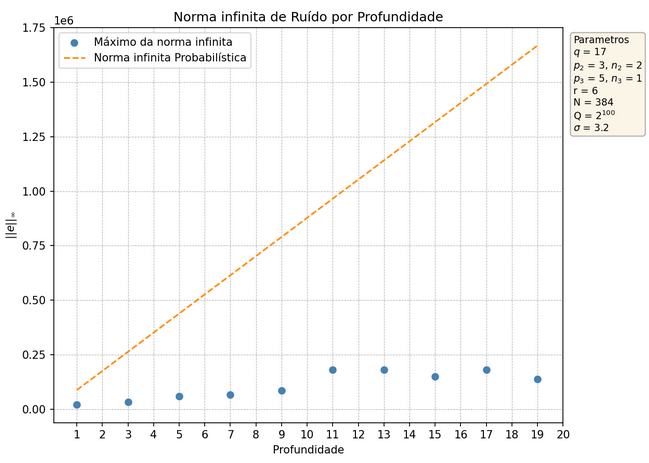
\includegraphics[width=\linewidth]{sections/images/image2.png}
  \end{subfigure}
  \hfill
  \begin{subfigure}{0.45\textwidth}
    \centering
    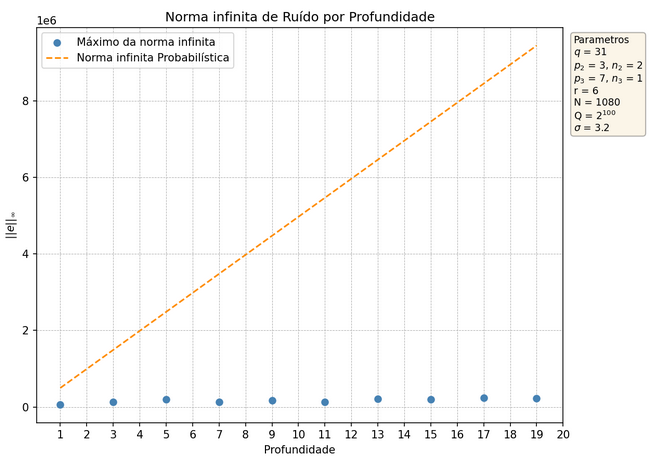
\includegraphics[width=\linewidth]{sections/images/image.png}
  \end{subfigure}
  \caption{Gráficos da norma infinita pela quantidade de produtos externos realizados }
\end{figure}

Para a geração destes \emph{plots} foram omitidas as constantes dos primos, levou-se em conta apenas as variáveis relacionadas ao parâmetro de segurança, $O(r^3\sqrt{N\log Q}E)$. Perceba que mesmo assim, existe uma distância bem razoável entre o ruído encontrado e o limite probabilistíco encontrado. Dado estes e outros testes, é um bom indicativo que escolher os parâmetros da forma utilizada pelo artigo, com a constante da análise assintótica sendo $1$ é, de fato, condizente com a realidade.



\subsection{Complexidades}
Para a memória, é trivial que um inteiro com tamanho máximo $Q$ pode ser representado por $\log Q$ bits, disto, segue que um  polinômio de grau $N$ com seus coeficientes em $\mathbb{Z}_Q$ é representado por $O(N \log Q)$ bits. Na implementação realizada fica claro que a complexidade de memória do \emph{framework} é $O(r N \log^2 Q)$ que provém das chaves de bootstrapping, em que cada criptograma tem $O(N \log^2Q)$ bits armazenando $r$ mensagens, valores idênticos ao desenvolvido anteriormente, por exemplo em \cite{Guimaraes2023Amortized}. 

Para complexidade temporal, a parte relevante para este trabalho é a do produto externo definido pelo trabalho analisado. A complexidade do \textit{produto externo padrão} envolve, primeiramente, a decomposição de dois polinômios. Em seguida, executa-se a multiplicação de um vetor $(1 \times 2\ell)$ por uma matriz $(2\ell \times 2)$, cujos elementos são polinômios com coeficientes de até $N \log Q$ bits. Essa etapa requer $4\ell$ multiplicações polinomiais e $4\ell - 2$ somas polinomiais, resultando na complexidade final $O(N \log N \log^2 Q)$.
 
No \textbf{traço homomórfico}, além de um produto externo, são realizadas $\log r$ chamadas de \textit{key-switch} em que cada uma tem duas aplicações de automorfismo. Cada key-switch demanda uma decomposição polinomial, $2\ell$ multiplicações polinomiais e $2\ell-2$ somas polinomiais. Agregando isto, por cada produto interno no framework proposto temos $[(2\ell-2) \log r + 8\ell - 2]$ somas polinomiais, $[2\ell \log r + 8\ell]$ multiplicações polinomiais, $(2 \log r)$ automorfismos e $(\log r + 2)$ decomposições. Ao utilizarmos as complexidades mais favoráveis obtemos $O(N \log N \log r \log^2 Q )$, substituindo pelos parâmetros propostos $\tilde{O}(\lambda \log ^3 \lambda \log r)$ por produto externo de $r$ mensages, resultando em uma complexidade amortizada $\tilde{O}(\log ^4 \lambda) \cong \tilde{O}(1)$ em contraste de $O(\lambda \log^3 \lambda) \cong \tilde{O}(\lambda)$ obtido pelo TFHE apresentado em \cite{Guimaraes2023Amortized}.

\subsection{Comentário final}
A implementação atual ainda não é capaz de explorar plenamente todo o potencial teórico do \textit{framework} proposto. Há diversas otimizações possíveis, como o uso de NTTs mais otimizadas, a substituição do módulo $Q$ por um primo adequado, decomposições mais eficientes, uso de CRT, pré-computação dos automorfismos na base (com \textit{trade-off} de memória), entre outras técnicas possíveis descritas em artigos \cite{lw23II, lyubashevsky2013}. Apesar dessas limitações, a presente implementação serve como guia e demonstra resultados promissores, especialmente pelo bom comportamento observado no ruído. Com a aplicação das otimizações mencionadas, será possível quantificar com precisão as constantes associadas ao produto externo proposto. No entanto, na implementacão atual, o novo método ainda é mais lento, na prática, quando comparado a outros produtos externos amortizados do estado da arte, como em \cite{Guimaraes2023Amortized}. Assim, uma implementação otimizada é indispensável para garantir uma comparação justa e fidedigna com tais abordagens. 
